\chapter{ГЛАВА 3. ОПИСАНИЕ ПРОЦЕССА МОДЕЛИРОВАНИЯ}
\label{ch:chapter3}
\section{Связь моделирования и симуляции. Имитация датчика температуры}

Моделирование $-$ это процесс создания модели объекта или системы, которая может быть использована для анализа, прогнозирования и оптимизации поведения объекта или системы. Моделирование может быть как математическим, так и физическим.

Симуляция $-$ это процесс имитации реального объекта или события в виртуальной среде. Симуляция использует модели для создания виртуальной среды и позволяет исследовать различные сценарии и принимать решения без риска потери жизни или материальных ценностей.

Т. е., моделирование является более широким понятием, которое включает в себя создание моделей, анализ и оптимизацию поведения объекта или системы, а симуляция является одним из инструментов моделирования, который позволяет проводить имитацию реальных объектов или событий в виртуальной среде. Моделирование и симуляция процессов в физике $-$ это важный инструмент для изучения и понимания физических явлений. Они позволяют создавать математические модели, которые могут быть использованы для прогнозирования поведения системы в различных условиях.

Большая часть данной работы посвящена визуальному моделированию, которое может быть полезно в обучении и просто для лучшего понимания физических процессов. Однако как уже говорилось ранее, это не единственный вид моделирования, помимо прочего есть также математическое моделирование, которое позволяет нам правильно описывать физические процессы для того, чтобы  в дальнейшем использовать в различных исследованиях или в том же визуальном моделировании объектов.

Симуляция поведения различных объектов, утсройств может быть также использована для настройки, отладки и тестирования программы, прогнозирования ее поведения в тех или иных случаях. Рассмотрим управляющую программу контроллера. Но сперва дадим определения понятиям:

\begin{itemize}
    \item Контроллер $-$ это устройство, которое управляет работой других устройств или систем. Он может быть программным или аппаратным, и его задача $-$ обеспечить координацию и контроль работы других устройств.
    \item Аналоговые устройства $-$ это устройства, которые работают с непрерывными сигналами, такими как напряжение или ток. Они используются для обработки и управления аналоговыми сигналами, например, для управления скоростью двигателя или регулирования яркости света.
    \item Датчик температуры $-$ это устройство, которое измеряет температуру в окружающей среде или внутри объекта и преобразует ее в сигнал, который может быть использован для контроля и регулирования температуры.
\end{itemize}

Контроллеры и аналоговые устройства $-$ это ключевые элементы в многих технических системах, которые используются для управления и контроля различных процессов. Они играют важную роль в автоматизации производственных процессов, управлении энергосистемами и других технических системах. Управляющую программу можно запускать в режиме эмуляции или напрямую подключенную к контроллеру с аналоговым устройством. Режим эмуляции помогает отладить и протестировать некоторые функции программы без дополнительных подключений. В нашем примере в качестве аналогвого устойства будет рассмотрен датчик температуры, вернее его имитация при запуске приложения в режиме эмуляции.

Существует несколько причин, по которым программы для контроллеров могут быть запущены в режиме эмуляции:

\begin{enumerate}
    \item Тестирование: эмуляция позволяет тестировать программы для контроллеров без необходимости иметь физический контроллер. Это может быть полезно для разработчиков, которые могут проверить, как программа работает на разных типах контроллеров.
    \item Обучение: эмуляция может быть использована для обучения студентов или новых сотрудников, которые должны знать, как работать с программами для контроллеров.
    \item Экономия времени и денег: эмуляция может сэкономить время и деньги, которые могут быть потрачены на покупку и установку физического контроллера.
    \item Удобство: эмуляция может быть более удобной для тех, кто работает с программами для контроллеров на удаленном компьютере или в виртуальной среде.
\end{enumerate}

Проект с управляющей программой находится по ссылке\footnote{\scriptsize{https://github.com/savushkin-r-d/ptusa\_main.}}. Файлы с реализацией analog\_emulator.h и analog\_emulator.cpp находятся в папке ptusa\_main/Pac/common. Код написан на языке программирования C++, 11 стандарта. Данный стандарт выбран в целях оптимизации на различных платформах. В программе значения температуры генерируются согласно функции нормального распределения. При необходимости логику генерации чисел в дальнейшем можно менять.

Нормальное распределение $-$ непрерывное распределение вероятностей с пиком в центре и симметричными боковыми сторонами, которое в одномерном случае задаётся функцией плотности вероятности, совпадающей с функцией Гаусса:

$$ f(x)= \frac{1}{\sigma \sqrt{2\pi}} \: e^{-{\frac{1}{2}}{\left(\frac{x-\mu}{\sigma}\right)}^2} \eqno (3.1.1)$$

\noindent где ${\mu}$ $-$ математическое ожидание, $\sigma$ $-$ среднеквадратичное отклонение, $\sigma^2$ $-$ дисперсия распределения.

Математическое ожидание ${\mu}$ $-$ среднее значение случайной величины в результате многократного повторения.

В классе analog\_emulator определены методы get\_st\_deviation(), get\_m\_expec() возвращают значения стандартного отклонения и математического ожидания. Математическое ожидание и стандартное отклонение задаются в параметрах конструктора.

Метод  get\_value() c помощью объектов класса std::random\_device (генерирует равномерно распределенные целые случайные числа) и std::normal\_distribution (генерирует случайные числа согласно нормальному распределению) возвращает значения температуры. Математическое ожидание и стандартное отклонение $-$ параметры конструктора std::normal\_distribution. Чтобы в дальнейшем иметь возможность изменить параметры в analog\_emulator определен метод param , который принимает в качестве аргументов новые значения математического ожидания и стандартного отклонения.

\section{Моделирование распределения частиц в поле силы тяжести}

Моделирование реализовано на языке прграммирвания JavaScript и элементом HTML5 Canvas. Для работы с Canvas необходимо сперва задать тег в html документе c указанием размеров окна.

\begin{minted}[
frame=single,
framesep=5mm,
baselinestretch=1.2,
%bgcolor=LightGray,
fontsize=\scriptsize,
]{html}
<canvas id="canvas" width="700" height="700"></canvas>
\end{minted}

\noindent Затем в JavaScript коде настроить поле для рисования.

\begin{listing}[H]
\begin{minted}
[
frame=single,
framesep=1mm,
fontsize=\scriptsize,
]{js}
var canvas = document.getElementById('canvas');
var context = canvas.getContext('2d');
var canvas_bg = document.getElementById('canvas_bg');
var context_bg = canvas_bg.getContext('2d');
\end{minted}
\end{listing}

\noindent Объявляем переменные, которые будут использоваться в процессе моделирования.

\begin{listing}[H]
\begin{minted}
[
frame=single,
framesep=1mm,
fontsize=\scriptsize,
]{js}
var particles; // частицы
var numParticles = 300; // количество частиц
var walls; // стенки сосуда
var t0, dt; // время для точного расчета движения
var g = 15; // гравитация
var force; // силы
var acc; // ускорение
\end{minted}
\end{listing}

\noindent Присваиваем функцию init() в качестве обработчика события onload объекта window.

\begin{listing}[H]
\begin{minted}
[
frame=single,
framesep=1mm,
fontsize=\scriptsize,
]{js}

window.onload = init;

\end{minted}
\end{listing}

\noindent Функция init() будет вызвана автоматически после того, как страница будет полностью загружена. Это позволяет гарантировать, что все элементы страницы будут доступны для работы с ними в функции init().
В функции init():

\noindent 1. Задание радиуса частицы.

\begin{listing}[H]
\begin{minted}
[
frame=single,
framesep=1mm,
fontsize=\scriptsize,
]{js}

var radius = 7;

\end{minted}
\end{listing}

\noindent 2. Инициализация скорости по $x$ и $y$ случайными значениями в диапазоне от 0 до 10.

\begin{listing}[H]
\begin{minted}
[
frame=single,
framesep=1mm,
fontsize=\scriptsize,
]{js}

var speed_x = getRandomArbitrary(0, 10);
var speed_y = getRandomArbitrary(0, 10);

\end{minted}
\end{listing}

\noindent 3. Расчет массы частицы.

\begin{listing}[H]
\begin{minted}
[
frame=single,
framesep=1mm,
fontsize=\scriptsize,
]{js}

var mass = 0.01*Math.pow(radius,3);

\end{minted}
\end{listing}

\noindent 4. Создание объекта Particle, а также векторов с координатами позиции и скорости частицы.

\begin{listing}[H]
\begin{minted}
[
frame=single,
framesep=1mm,
fontsize=\scriptsize,
]{js}
var particle = new Particle(radius,'#5C62D6',mass,0);
var particle = new Particle(radius,'#5C62D6',mass,0); // создаем объект Particle
particle.pos2D = new Vector2D(Math.random()*(canvas.width-2*radius)+radius,
                          Math.random()*(canvas.height-2*radius)+radius);
                          // вектор с координатами позиции частицы x,y
particle.velo2D = new Vector2D(speed_x, speed_y);// вектор с координатами скорости по x и y
\end{minted}
\end{listing}

\noindent 5. Добавление частицы в массив и вызов метода для ее отрисовки.

\begin{listing}[H]
\begin{minted}
[
frame=single,
framesep=1mm,
fontsize=\scriptsize,
]{js}

particles.push(particle);
particle.draw(context);

\end{minted}
\end{listing}

\noindent Реализация построения объекта Particle находится в файле \\ /gravity/objects/particle.js. Нам нужно создать свойства объекта на основе физических параметров, таких как масса, заряд, положение и скорость. Мы должны иметь возможность cчитывать, а также изменять эти параметры. Мы создаем векторы положения и скорости pos2D и velo2D как объекты Vector2D из их соответствующих компонентов. Реализация этих свойств происходит следующим образом. Для начала мы определяем массу частицы, заряд, свойства $x$, $y$, $v_x$ и $v_y$ в ее конструкторе:

\begin{listing}[H]
\begin{minted}
[
frame=single,
framesep=1mm,
fontsize=\scriptsize,
]{js}
function Particle(mass,charge){
 if(typeof(mass)==='undefined') mass = 1;
 if(typeof(charge)==='undefined') charge = 0;
 this.mass = mass;
 this.charge = charge;
 this.x = 0;
 this.y = 0;
 this.vx = 0;
 this.vy = 0;
}
\end{minted}
\end{listing}

\noindent Свойства pos2D и velo2D  добавляются к прототипу частиц с помощью геттеров и сеттеров:

\begin{listing}[H]
\begin{minted}
[
frame=single,
framesep=1mm,
fontsize=\scriptsize,
]{js}
Particle.prototype = {
 get pos2D (){
 return new Vector2D(this.x,this.y);
 },
 set pos2D (pos){
 this.x = pos.x;
 this.y = pos.y;
 },
 get velo2D (){
 return new Vector2D(this.vx,this.vy);
 }

 set velo2D (velo){
 this.vx = velo.x;
 this.vy = velo.y;
 }
}
\end{minted}
\end{listing}

Чтобы упростить код для обновления значения pos2D и velo2D частицы, были добавлены методы, multiply(k) и addScaled(vec, k), к объекту Vector2D (где vec $-$ это Vector2D, а $k$ $-$ число). Метод vec1.multiply(k) умножает вектор vec1 на скаляр $k$, а vec1.addScaled(vec, k) добавляет $k$ раз vec к vec1.

Наличие столкновений между парами частиц в массиве проверяются в методе checkCollision(). Для этого мы используем Vector2D.distance(vec1,vec2), статический метод, который вычисляет расстояние между двумя точками с помощью векторов положения vec1 и vec2.

\begin{listing}[H]
\begin{minted}
[
frame=single,
framesep=1mm,
fontsize=\scriptsize,
]{js}
// STATIC METHODS
Vector2D.distance =  function(vec1,vec2){
  return (vec1.subtract(vec2)).length();
}
\end{minted}
\end{listing}

Логика алгоритма обнаружения столкновений проста: если расстояние между центрами двух частиц меньше или равно сумме их радиусов, это означает, что они столкнулись. Затем мы меняем местами скорости двух частиц. \cite{canvas14}

Все необходимые методы для работы с векторами находятся в файле /gravity/objects/vector2D.js. Среди них:

\begin{itemize}
    \item Расчет длины вектора
    \item Сложение и вычитание векторов
    \item Умножение вектора на скаляр
    \item Скалярное произведение векторов
    \item Вычисление проекции вектора vec1 в направлении вектора vec2.
    \item Вычисление расстояния и угла между двумя векторами
\end{itemize}

JavaScript для анимации использует функции таймера. Самые популярные из них это setTimeout() и setInterval(). Данные методы используются для управления временем выполнения кода. setTimeout() позволяет задержать выполнение функции на определенный промежуток времени (в миллисекундах). Он принимает два аргумента: функцию, которую нужно выполнить, и время задержки.

setInterval() позволяет запускать функцию через определенные промежутки времени. Он также принимает два аргумента: функцию, которую нужно выполнить, и время задержки между ее запусками. Мы можем указать задержку времени в функции setInterval() как $1000$ / fps, где fps $-$ это частота кадров анимации, то есть количество обновлений или кадров в секунду. Как частота кадров связана с воспринимаемой скоростью анимации? Чтобы ответить на этот вопрос, нам нужно выполнить некоторые простые математические операции. Предположим, что мы хотим перемещать объект с постоянной скоростью $100$ пикселей в секунду, и предположим, что частота кадров анимации составляет $50$ кадров в секунду. Давайте увеличим горизонтальную позицию объекта на $v_x$ за кадр, как в примере отскакивающего мяча:

\begin{listing}[H]
\begin{minted}
[
frame=single,
framesep=1mm,
fontsize=\scriptsize,
]{js}
function onEachStep() {
 ball.x += vx;
}
\end{minted}
\end{listing}

Другими словами, $v_x$ $-$ это горизонтальная скорость в единицах пикселей за кадр. Скорость в единицах пикселей в секунду равна $100$, а количество кадров в секунду равно $50$. Таким образом, значение $v_x$ равно $100/50$ или $2$. В общем случае у нас есть следующее соотношение: (Скорость в пикселях в секунду) = (Скорость в пикселях за кадр) $×$ (Частота кадров в кадрах в секунду). Если установить $v_x = 2$, мы должны увидеть, что мяч движется со скоростью $100$ пикселей в секунду. Скорость в пикселях в секунду $-$ это то, что мы фактически воспринимаем на экране. Однако нет гарантии, что частота кадров, на которой работает анимация, будет точно соответствовать установленной частоте кадров. Предположим, что ваш компьютер медленный или на нем запущено другое приложение, так что фактическая частота кадров ближе к $30$ кадрам в секунду. Это дает фактическую скорость только $60$ пикселей в секунду. Ваш объект кажется движущимся медленнее. Таким образом, установка частоты кадров в функции setInterval() не гарантирует скорость анимации. Чтобы попытаться решить эту проблему познакомимся с другим, более новым JavaScript методом анимации $-$ методом requestAnimationFrame(). \cite{canvas14}

В последние годы появилось новое API среди веб-браузеров, позволяющее разработчикам создавать анимации HTML5, которые получают преимущества от оптимизации, основанной на браузере, что позволяет значительно повысить производительность по сравнению со старыми методами setInterval() и setTimeout().

requestAnimationFrame() используется для анимации и обновления интерфейса. Он запускает функцию на следующем кадре анимации, что позволяет браузеру оптимизировать процесс обновления интерфейса и избежать проблем с частотой кадров. Функция requestAnimationFrame(someFunction) вызывает функцию someFunction() перед перерисовкой экрана браузера. Некоторые реализации браузеров также включают второй параметр для указания элемента HTML5, к которому применяется перерисовка, например requestAnimationFrame(someFunction, canvas). Для создания цикла анимации с использованием requestAnimationFrame() достаточно включить его в функцию, которую он вызывает.

\begin{listing}[H]
\begin{minted}
[
frame=single,
framesep=1mm,
fontsize=\scriptsize,
]{js}
function animFrame(){
  animId = requestAnimationFrame(animFrame,canvas);
  onTimer();
}
\end{minted}
\end{listing}

Функция onTimer() содержит код анимации. Плохой учет времени может серьезно повлиять на физику. Для точного учета времени нам нужен способ измерения фактически прошедшего времени. К счастью, есть простой способ сделать это: использовать функцию getTime(). И этот метод можно использовать как с setInterval(), так и с requestAnimationFrame(). Функция getTime() является методом встроенного объекта JavaScript Date, и она возвращает целое число, равное количеству миллисекунд, прошедших с полуночи $1$ января $1970$ года. Таким образом, если вы вызовете Date.getTime() дважды в разных частях кода и вычислите разницу в возвращаемых значениях, то это даст вам время, прошедшее между этими двумя вызовами.
Как это помогает нам с анимацией? Суть в том, что мы можем вычислить фактическое время, прошедшее с момента последнего обновления позиции объекта. Затем мы можем использовать это время для вычисления величины, на которую нужно его переместить.
Рассмотрим реализицию функции onTimer().

\begin{listing}[H]
\begin{minted}
[
frame=single,
framesep=1mm,
fontsize=\scriptsize,
]{js}
function onTimer(){
  var t1 = new Date().getTime();
  dt = 0.001*(t1-t0);
  t0 = t1;
  if (dt>0.2) {dt=0;};
  move();
}
\end{minted}
\end{listing}

Первая строка получает текущее время в миллисекундах, вызывая Date().getTime(). Вторая строка вычисляет прошедшее время $dt$ в секундах с последнего вызова onTimer(). Здесь $t_0$ $-$ это переменная, инициализированная как new Date().getTime() перед началом анимации в функции Init(). Следующая строка сбрасывает $t_0$, чтобы его можно было использовать для следующего вызова.

За создание стенок сосуда отвечает объект Wall. Его реализация находится в файле /gravity/objects/wall.js. Объект Wall $-$ это простой объект, который рисует линию между двумя указанными конечными точками. Конечными
точками являются объекты Vector2D. Отрисовка и создание объекта Wall также как и частицы происходит в методе Init():

\begin{listing}[H]
\begin{minted}
[
frame=single,
framesep=1mm,
fontsize=\scriptsize,
]{js}
walls = new Array();
var wall1 = new Wall(new Vector2D(canvas.width,0),new Vector2D(0,0));
wall1.draw(context_bg);
wall1.draw(context_bg);
walls.push(wall1);
\end{minted}
\end{listing}

\noindent Расчет силы тяжести, действующей на частицу, осуществляет метод CalcForce().

\begin{listing}[H]
\begin{minted}
[
frame=single,
framesep=1mm,
fontsize=\scriptsize,
]{js}
function calcForce(obj){
  force = Forces.constantGravity(obj.mass,g);
}
\end{minted}
\end{listing}

\noindent Метод constantGravity() находится в файле /gravity/objects/forces.js.
\begin{listing}[H]
\begin{minted}
[
frame=single,
framesep=1mm,
fontsize=\scriptsize,
]{js}
Forces.constantGravity = function(m,g){
  return new Vector2D(0,m*g);
}
\end{minted}
\end{listing}

\noindent Как видно в листинге выше в качестве параметров он принимает значения массы и силы тяжести.

\newpage
\section{Моделирование распределения молекул по скоростям}

Программа моделирует систему частиц и анимированную гистограмму распределения их скоростей, используя модули matplotlib и numpy. Код разделен на 3 файла:

\begin{enumerate}
    \item main.py
    \item particle.py
    \item histogram.py
\end{enumerate}

В файлах particle.py и histogram.py реализованы классы Particle и Histogram, которые отвечают за настройку параметров частиц и гистограммы. В Matplotlib гистограмма представлена как набор прямоугольников (столбцов), патчами (patches). Каждый патч представляет собой один столбец гистограммы и имеет свои свойства.

Класс matplotlib.hist.patch используется для создания и настройки патчей гистограммы. Он содержит методы для установки свойств патча, таких как set\_facecolor() для установки цвета заполнения патча, set\_alpha() для установки прозрачности и т.д.

В данной программе гистограмма и ее параметры описаны в классе Histogram. Инициализатор класса строит гистограмму передавая в  np.histogram значения скоростей частиц, количество столбцов,  а также булевый параметр density. В matplotlib.pyplot.hist параметр
density позволяет нормировать гистограмму так, чтобы площадь под ней была равна 1.

\begin{minted}
[
frame=single,
framesep=1 mm,
baselinestretch=1.2,
fontsize=\scriptsize,
]
{python}

self.hist, bins = np.histogram(data, self.bins, density=density)

\end{minted}

Метод draw() отрисовывает гистограмму, а метод update() перестраивает гистограмму согласно новым данным значений скоростей после столкновения частиц друг с другом. В классе Particle происходит инициализация параметров частиц, таких как масса, радиус, первоначальное положение и скорость.

\begin{minted}
[
frame=single,
framesep=1 mm,
baselinestretch=1.2,
fontsize=\scriptsize,
]
{python}
def __init__(self, pos, vel, r, m):
        self.pos = np.asarray(pos, dtype=float)
        self.vel = np.asarray(vel, dtype=float)
        self.n = self.pos.shape[0]
        self.r = r
        self.m = m
\end{minted}

\noindent Также данный класс просчитывает столкновения частиц друг с другом и со стенками сосуда. Метод def advance() обновляет позицию частиц в соответствии с их скоростями.

\begin{minted}
[
frame=single,
framesep=1 mm,
baselinestretch=1.2,
fontsize=\scriptsize,
]
{python}

self.pos += self.vel * dt

\end{minted}

Для расчета столконовений в Particle импортируются функции pdist и squareform модуля scipy.spatial.distance библиотеки SciPy.

\begin{minted}
[
frame=single,
framesep=1 mm,
baselinestretch=1.2,
fontsize=\scriptsize,
]
{python}

from scipy.spatial.distance import pdist, squareform

\end{minted}

\noindent pdist $-$ это функция, которая вычисляет попарные расстояния между точками в пространстве. Она принимает на вход массив точек и возвращает массив расстояний между всеми парами точек.
squareform $-$ это функция, которая преобразует массив попарных расстояний, полученный с помощью pdist, в квадратную матрицу расстояний. Она принимает на вход массив попарных расстояний и возвращает квадратную матрицу расстояний.

В файле main.py настраивается окно вывода Matplotlib.

\begin{minted}
[
frame=single,
framesep=1 mm,
baselinestretch=1.2,
fontsize=\scriptsize,
]
{python}
DPI = 100
width, height = 1000, 500
fig = plt.figure(figsize=(width/DPI, height/DPI), dpi=DPI)
fig.subplots_adjust(left=0, right=0.97)
sim_ax = fig.add_subplot(121, aspect='equal', autoscale_on=False)
sim_ax.set_xticks([])
sim_ax.set_yticks([])
speed_ax = fig.add_subplot(122)
speed_ax.set_xlabel('Speed $v\,/m\,s^{-1}$')
speed_ax.set_ylabel('$f(v)$')
\end{minted}

\noindent Создаются объекты классов Particle и Histogram.

\begin{minted}
[
frame=single,
framesep=1 mm,
baselinestretch=1.2,
fontsize=\scriptsize,
]
{python}
sim = Particle(pos, vel, r, m)
speed_hist = Histogram(speeds, 2 * sbar, 50, density=True)
\end{minted}

Для моделирования частиц в программе используются также matplotlib.patches. Класс ParticlePatch в модуле matplotlib.patches используется для создания патчей, представляющих частицы в системах. Он позволяет задавать различные параметры частиц, такие как размер, цвет и положение на графике. ParticlePatch может быть полезен в различных областях, таких как физика, химия и материаловедение, где важно визуализировать системы частиц и их поведение на графике. \cite{PLOTD}
\newpage
Анимацию в Matplotlib удобно осуществлять с помощью FuncAnimation().

\begin{minted}
[
frame=single,
framesep=1 mm,
baselinestretch=1.2,
fontsize=\scriptsize,
]
{python}
frames = 800
anim = FuncAnimation(fig, animate, frames=frames, interval=45, init_func=init_anim)
\end{minted}

\noindent FuncAnimation() для анимации необходимы

\begin{minted}
[
frame=single,
framesep=1 mm,
baselinestretch=1.2,
fontsize=\scriptsize,
]
{python}
fig       #объект, фигура на которой будет производиться отрисовка
animate() #функция, которая будет вызываться для каждого кадра
frames    #количество кадров
interval  #задержка между кадрами в мс
init_func #функция для отрисовки четкого кадра
\end{minted}

\noindentЕсли init\_func не указана, будут использованы результаты рисования из первого элемента в последовательности кадров.

Функция animate() вызывает методы advance() для обновления позиции частиц и get\_speeds() для получения скоростей, которые дальше передаются  в метод update() класса Histogram.

\begin{minted}
[
frame=single,
framesep=1 mm,
baselinestretch=1.2,
fontsize=\scriptsize,
]
{python}
def animate(i):
    global sim, verts, mb_est_line, mb_est
    sim.advance(dt)

    particles.set_data(sim.pos[:, X], sim.pos[:, Y])
    particles.set_markersize(10) # размер частицы

    speeds = get_speeds(sim.vel)
    speed_hist.update(speeds)
\end{minted}

\noindent get\_speeds() считает магнитуду. \cite{MD}

\begin{minted}
[
frame=single,
framesep=1 mm,
baselinestretch=1.2,
fontsize=\scriptsize,
]
{python}
def get_speeds(vel):
    return np.hypot(vel[:, X], vel[:, Y])
\end{minted}
\newpage
\section{Моделирование броуновского движения}

Моделирование осуществляется с помощью Pygame и Pymunk. Параметры атомов описаны в классе Atom. Данный класс имеет такие поля как радиус, скорость, масса, плотность, упругость, форму, начальную позицию и координаты.

\begin{minted}
[
frame=single,
framesep=1 mm,
baselinestretch=1.2,
fontsize=\scriptsize,
]
{python}
class Atom():
    def __init__(self,x,y):
        self.x=x
        self.y=y
        self.mass=1
        self.radius=8
        self.moment=pymunk.moment_for_circle(self.mass,0,self.radius)
        self.body=pymunk.Body(self.mass,self.moment)
        self.body.position=x,y
        self.body.velocity=random.uniform(-100,100),random.uniform(-100,100)
        self.shape=pymunk.Circle(self.body,self.radius)
        self.shape.density=1
        self.shape.elasticity=1
        space.add(self.body,self.shape)
\end{minted}

\noindent Класс имеет один метод, который в качестве параметра принимает объект класса Atom и с помощью его координат с радиусом  рисует фигуру на поверхности. Отрисовка производится посредством встроенного в Pygame метода draw.circle().

\begin{minted}
[
frame=single,
framesep=1 mm,
baselinestretch=1.2,
fontsize=\scriptsize,
]
{python}
def draw(self):
    x,y=self.body.position
    pygame.draw.circle(display,PURPLE,(int(x),int(y)),self.radius)
\end{minted}

Модель частицы описана в классе Particle, который идентичен классу Atom. Отличие двух классов заключается в значениях таких полей как радиус, масса, скорость и плотность. Здесь также присутствует метод класса draw(), который принимает в качестве параметра объект класса Particle.
Классы описывают модель одного атома или частицы вещества. Но нам нужно, чтобы этих частиц было много и вообще для начала их создать.
Данный процесс происходит в функции game(), в которой создаются объекты всех вышеперечисленных классов, а также в функции game() находится главный цикл, который будет вызывать все методы для отрисовки физических объектов.
Функция game() не принимает никаких параметров на входе. В её реализации прописано создание списков объектов классов Atom, Particle и Wall. Списки генерируются с помощью механизма языка Python list comprehension. Это нужно, чтобы происходила отрисовка не одной, а множества частиц на экране.
\newpage
\begin{minted}
[
frame=single,
framesep=1 mm,
baselinestretch=1.2,
fontsize=\scriptsize,
]
{python}
def game():
    atoms=[Atom(random.randint(0,800),random.randint(0,800)) for i in range(450)]
    particles=[Particle(random.randint(0,800),random.randint(0,800)) for i in range(5)]
    walls=[Wall((0,0),(0,800)),
    Wall((0,0),(800,0)),
            Wall((0,800),(800,800)),
            Wall((800,0),(800,800))]
    while True:
        for event in pygame.event.get():
        if event.type==pygame.QUIT:
           exit()

        display.fill((0,0,0))
        for atom in atoms:
            atom.draw()
            for particle in particles:
                particle.draw()

        pygame.display.update()
        clock.tick(FPS)
        space.step(1/FPS)
\end{minted}

\newpage

\section{Результаты моделирования}

  \begin{figure}[ht]
 \centering
		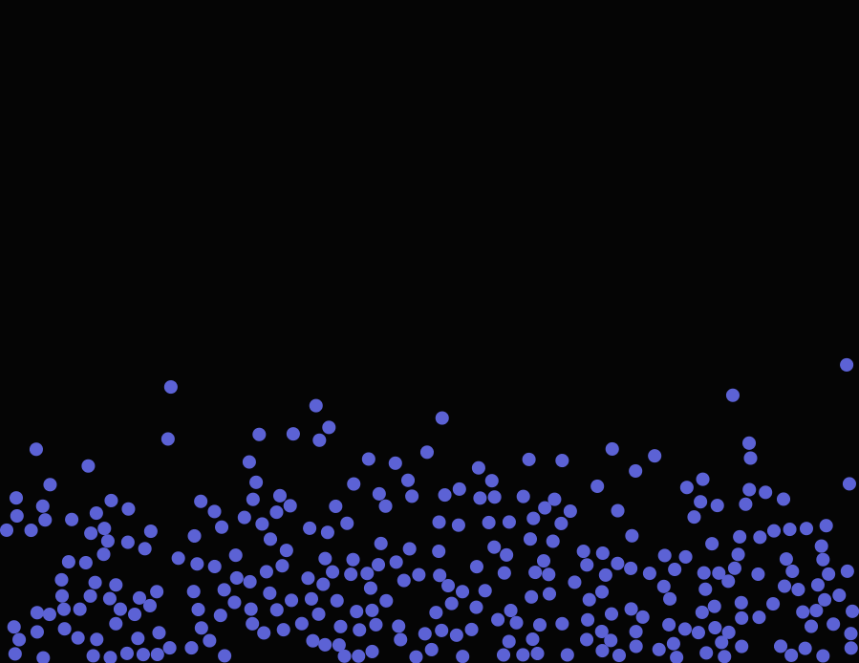
\includegraphics[height =11 cm, keepaspectratio]{images/gravity.png}
		\caption{ \textbf{Рис. 3.5.1.} Распределение молекул в поле силы тяжести}
	\end{figure}
 \begin{figure}[ht]
 \centering
		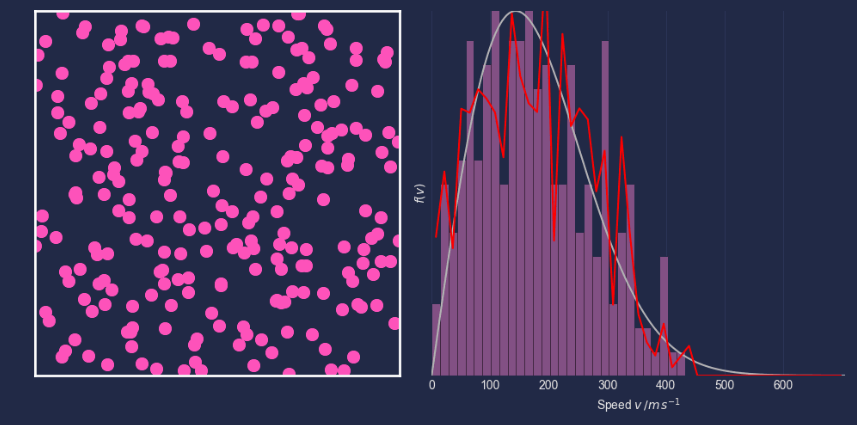
\includegraphics[height =8 cm, keepaspectratio]{images/maxwell_boltsman.png}
		\caption{ \textbf{Рис. 3.5.2.} Распределение молекул по скоростям}

	\end{figure}

\begin{figure}[ht]
 \centering
		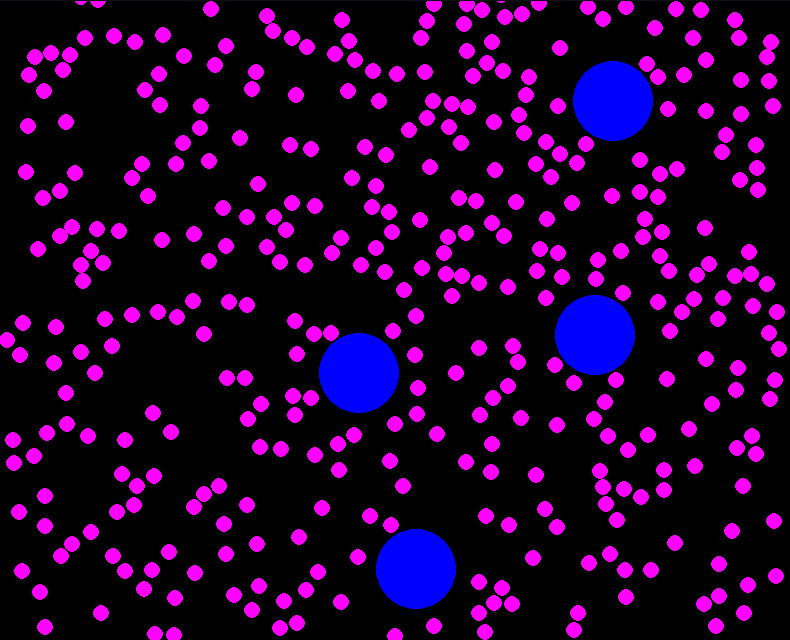
\includegraphics[height =15 cm, keepaspectratio]{images/brownian.png}
		\caption{ \textbf{Рис. 3.5.3.} Броуновское движение}
	\end{figure}
 \hfill








